% ==========================================
% BAB I PENDAHULUAN
% ==========================================
\chapter{PENDAHULUAN}
\label{chap:pendahuluan}
% --- Latar Belakang ---
\section{Latar Belakang}

Transformasi digital di sektor bisnis telah mengubah cara perusahaan menganalisis dan memanfaatkan data untuk pengambilan keputusan strategis. \textit{Business Intelligence} (BI)\label{abbr:BI} kini menjadi tulang punggung operasional organisasi modern yang ingin tetap kompetitif di pasar global. Pasar global \textit{Business Intelligence} diproyeksikan mencapai USD 36{,}82 miliar pada tahun 2025 dan tumbuh menjadi USD 116{,}25 miliar pada tahun 2033, dengan tingkat pertumbuhan tahunan gabungan (CAGR)\label{abbr:CAGR} sebesar 14{,}98\% \autocite{Straits2024}. Pertumbuhan ini menunjukkan bahwa organisasi di seluruh dunia semakin menyadari nilai strategis sistem analitik berbasis data untuk meningkatkan efisiensi operasional dan daya saing.

Di Indonesia, adopsi teknologi kecerdasan buatan (\textit{Artificial Intelligence}/AI)\label{abbr:AI} dan digitalisasi juga mengalami akselerasi signifikan. Laporan industri mencatat bahwa tingkat adopsi AI di kalangan pelaku bisnis Indonesia terus meningkat, meskipun sebagian besar masih pada tahap pemanfaatan dasar untuk efisiensi operasional \autocite{EastVC2025}. Tren ini sejalan dengan temuan global bahwa organisasi yang mengadopsi pengambilan keputusan berbasis data memperoleh keunggulan produktivitas yang terukur dibandingkan organisasi yang belum mengadopsinya \autocite{Brynjolfsson2016DDD}.

Salah satu tantangan utama dalam implementasi BI adalah kompleksitas akses dan interpretasi data bagi pengguna nonteknis. Sistem BI konvensional sering memerlukan keahlian khusus dalam bahasa kueri (seperti SQL\label{abbr:SQL}) dan pemahaman mendalam tentang struktur basis data sehingga menjadi hambatan bagi manajer dan staf operasional yang membutuhkan \textit{insight} cepat untuk keputusan harian. Dalam mengatasi hal tersebut, teknologi \textit{Conversational AI} berbasis \textit{chatbot} muncul sebagai solusi yang menjanjikan. Pasar \textit{Conversational AI} global diperkirakan mencapai USD 49{,}7 miliar pada tahun 2025 dan tumbuh dengan CAGR sekitar 23{,}6\% hingga 2032 \autocite{Qaltivate2025}.

Implementasi \textit{chatbot} dalam konteks layanan pelanggan dan operasional internal telah menunjukkan hasil yang positif. Penelitian menunjukkan bahwa \textit{chatbot} berbasis AI mampu menangani sebagian besar pertanyaan rutin pelanggan secara otomatis, mempercepat waktu respons, dan mengurangi beban kerja agen manusia secara signifikan \autocite{Adam2021Chatbots}. Dalam konteks BI, \textit{chatbot} berfungsi sebagai antarmuka percakapan yang memungkinkan pengguna internal, seperti manajer penjualan, tim layanan pelanggan, dan analis bisnis, mengakses data analitik, laporan, dan prediksi melalui kueri bahasa alami tanpa keahlian teknis. Studi \autocite{Iqbal2021} menunjukkan bahwa penerapan \textit{natural language processing} (NLP)\label{abbr:NLP} pada \textit{chatbot} meningkatkan efisiensi dan akurasi pelayanan pelanggan secara signifikan.

Teknologi NLP menjadi fondasi yang memungkinkan sistem memahami dan merespons kueri pengguna dalam bahasa alami. Pasar NLP global diproyeksikan tumbuh dari USD 35{,}43 miliar pada tahun 2024 menjadi USD 438{,}08 miliar pada tahun 2034, dengan CAGR sekitar 28{,}6\% \autocite{Precedence2025}. Dalam aplikasi BI, NLP memungkinkan sistem menginterpretasikan \textit{intent} pengguna, mengekstraksi entitas penting dari kueri, dan menghasilkan respons relevan berdasarkan konteks percakapan, baik melalui pendekatan \textit{rule-based} untuk kueri terstruktur maupun melalui model pembelajaran mesin untuk kueri yang lebih kompleks.

Selain kemampuan analisis deskriptif dan diagnostik, kebutuhan akan kemampuan prediktif dalam BI juga meningkat. Analisis prediktif memungkinkan organisasi mengantisipasi permintaan layanan pelanggan, merencanakan alokasi sumber daya, dan mengidentifikasi potensi \textit{churn} sebelum terjadi. Dalam konteks ini, permintaan layanan pelanggan didefinisikan sebagai minat, pesanan, dan kebutuhan pelanggan terhadap produk atau layanan yang ditawarkan perusahaan, yang dapat diukur melalui data pemesanan, target penjualan, tingkat \textit{churn}, dan pendapatan pelanggan. Pasar \textit{time series forecasting} secara global diperkirakan tumbuh dari sekitar USD 11{,}17 miliar (2024) menjadi USD 36{,}9 miliar pada 2032, dengan CAGR \mbox{$\sim$16{,}12\%} \autocite{WiseGuyReports2024}.

Metode \textit{forecasting} yang lazim meliputi model statistik dan model \textit{deep learning} untuk menangkap pola temporal. Pada kasus prediksi \textit{customer churn} di industri telekomunikasi, baik Random Forest maupun LSTM efektif dalam prediksi \textit{churn}, tetapi kegunaannya bergantung pada sifat data dan batasan bisnis. LSTM lebih baik bila interaksi pelanggan historis dan tren kepuasan menjadi kunci dalam pengambilan keputusan \autocite{Mena2023}.

Integrasi tiga komponen utama, \textit{Rule-Based Query}, \textit{Natural Language Generation}, dan \textit{Time Series Forecasting}, ke dalam satu sistem BI berbasis \textit{chatbot} menawarkan solusi komprehensif bagi kebutuhan analisis dan prediksi di lingkungan bisnis modern. Sistem demikian berpotensi memperkuat pengambilan keputusan proaktif berbasis data serta meningkatkan efisiensi operasional internal perusahaan.

% --- Rumusan Masalah ---
\section{Rumusan Masalah}

Sebagian besar sistem \textit{Business Intelligence} untuk analisis indikator permintaan terkait pelanggan di lingkungan internal perusahaan pada saat ini masih mengandalkan pelaporan manual, belum terintegrasi dengan antarmuka percakapan berbasis \textit{chatbot}, dan minim pemanfaatan kecerdasan buatan untuk analisis prediktif serta interaksi berbasis bahasa alami. Kondisi ini memunculkan sejumlah permasalahan sebagai berikut.

\begin{enumerate}
  \item \textbf{Keterbatasan akses analitik berbasis percakapan}
  
  Tidak tersedia sistem yang mampu memproses dan memahami permintaan data serta analisis bisnis secara otomatis dari pengguna internal melalui percakapan dalam bahasa alami. Hal ini menyebabkan pegawai mengalami kendala dalam memperoleh \textit{insight} terkait pesanan (\textit{order}), pencapaian target penjualan, \textit{churn} pelanggan, serta pendapatan secara cepat dan intuitif untuk mendukung pengambilan keputusan harian.

  \item \textbf{Ketiadaan fitur prediksi yang mudah diakses pengguna nonteknis}
  
  Belum terdapat fitur prediksi indikator utama bisnis terkait pelanggan, seperti peramalan jumlah pesanan, \textit{churn} pelanggan, dan target pendapatan berbasis pembelajaran mesin atau peramalan deret waktu yang dapat diakses oleh pengguna nonteknis. Keadaan ini menyebabkan perencanaan kapasitas, evaluasi target, dan penetapan strategi bisnis perusahaan menjadi kurang responsif terhadap tren serta dinamika bisnis pada masa yang akan datang.

  \item \textbf{Minimnya integrasi \textit{rule-based query} dan \textit{natural language generation}}
  
  Integrasi \textit{rule-based query} dan pemrosesan bahasa alami (\textit{natural language generation}) dalam sistem BI internal masih sangat terbatas sehingga proses pencarian data, penyaringan metrik utama, serta penyusunan laporan kinerja bisnis masih harus dilakukan secara manual dan berulang. Keadaan tersebut menimbulkan keterlambatan pengambilan keputusan serta penyajian data yang kurang selaras dengan kebutuhan analisis oleh manajemen.
\end{enumerate}

Bagaimana merancang dan mengembangkan sistem \textit{Business Intelligence} berbasis \textit{chatbot} yang terintegrasi dengan teknologi \textit{rule-based query}, pemrosesan bahasa alami dengan (\textit{natural language generation}), dan algoritma peramalan deret waktu sehingga seluruh pengguna internal perusahaan dapat menganalisis, memantau, dan memprediksi indikator bisnis pelanggan, seperti pesanan, target, \textit{churn}, dan pendapatan melalui antarmuka percakapan, serta memperoleh \textit{insight} berbasis data yang akurat, efisien, dan relevan untuk mendukung pengambilan keputusan bisnis dan perencanaan strategis perusahaan?

% --- Tujuan ---
\section{Tujuan}

Tujuan utama tugas akhir ini adalah merancang dan mengembangkan sistem \textit{Business Intelligence} berbasis \textit{chatbot} yang terintegrasi dengan teknologi \textit{rule-based query}, pemrosesan bahasa alami (\textit{Natural Language Generation}/NLG)\label{abbr:NLG}, dan algoritma peramalan deret waktu (\textit{time series forecasting}) untuk memfasilitasi pengguna internal perusahaan dalam menganalisis dan memprediksi indikator bisnis pelanggan.

Secara terperinci, tujuan yang hendak dicapai dalam tugas akhir ini adalah sebagai berikut.
\begin{enumerate}
  \item Merancang arsitektur sistem \textit{Business Intelligence} berbasis \textit{chatbot} yang mampu memproses permintaan analisis data dan memberikan \textit{insight} berbasis data kepada pengguna internal perusahaan secara otomatis.
  \item Mengimplementasikan modul pemrosesan bahasa alami sehingga pengguna internal dapat mengajukan pertanyaan dan permintaan analisis bisnis menggunakan bahasa alami melalui antarmuka \textit{chatbot}. 
  \item Mengimplementasikan modul mekanisme \textit{rule-based query} untuk menangani permintaan data yang bersifat terstruktur dan berulang dengan respons yang cepat dan konsisten.
  \item Mengintegrasikan model peramalan deret waktu (\textit{time series forecasting}) untuk menghasilkan prediksi terhadap indikator bisnis pelanggan, seperti volume pesanan, pencapaian target penjualan, tingkat \textit{churn} pelanggan, dan proyeksi pendapatan.
  \item Mengintegrasikan modul pembangkitan bahasa alami berbasis templat (\textit{template-based Natural Language Generation}) untuk menghasilkan narasi deskriptif dalam bahasa Indonesia dari data terstruktur hasil kueri basis data.
  \item Merancang dan mengimplementasikan antarmuka percakapan berbasis web yang mendukung interaksi bahasa alami, visualisasi peramalan interaktif, dan alur terpandu (\textit{guided flow}) bagi pengguna internal.
\end{enumerate}

% --- Batasan Masalah ---
\section{Batasan Masalah}

Dalam memfokuskan ruang lingkup penelitian dan memastikan kelayakan pelaksanaan tugas akhir, batasan-batasan penelitian ditetapkan sebagai berikut.
\begin{enumerate}
  \item Sistem dirancang khusus untuk pengguna internal perusahaan (manajer, analis bisnis, dan staf operasional), bukan untuk pelanggan eksternal.

  \item Sistem \textit{chatbot} hanya mendukung interaksi dalam Bahasa Indonesia.

  \item Sistem menggunakan data yang  terbatas pada data historis pelanggan yang mencakup informasi pesanan (\textit{order}), target penjualan, tingkat \textit{churn}, dan pendapatan dalam kurun waktu minimal dua tahun terakhir.

  \item Sistem hanya menangani permintaan terkait analisis deskriptif, diagnostik, dan prediktif terhadap indikator bisnis pelanggan. Sistem tidak mencakup fungsi transaksional atau modifikasi data.

  \item Sistem menggunakan metode peramalan deret waktu yang mencakup model \textit{deep learning} berupa LSTM\label{abbr:LSTM} (\textit{Long Short-Term Memory}) dan GRU\label{abbr:GRU} (\textit{Gated Recurrent Unit}), serta model statistik berupa ARIMA\label{abbr:ARIMA} (\textit{Autoregressive Integrated Moving Average}) dan Prophet sebagai \textit{baseline} pembanding. Model TFT\label{abbr:TFT} (\textit{Temporal Fusion Transformer}) dikaji pada tahap studi literatur dan perancangan, tetapi tidak diimplementasikan pada purwarupa ini dan dijadikan rekomendasi pengembangan di masa mendatang. Perbandingan antara model statistik dan model \textit{deep learning} dilakukan untuk menentukan pendekatan yang paling tepat sesuai dengan karakteristik data.

  \item Klasifikasi maksud pengguna (\textit{intent}) diimplementasikan dalam tujuh kategori utama (\textit{quantity}, \textit{trend}, \textit{comparison}, \textit{location}, \textit{performance}, \textit{detail}, \textit{reason}) beserta satu kategori cadangan (\textit{general}/\textit{fallback}). Setiap \textit{intent} dikombinasikan dengan delapan kategori fokus analisis dan dipetakan ke 38 aturan bisnis (\textit{business rules}) yang mencakup lima domain data.

  \item Sistem yang dikembangkan merupakan purwarupa mandiri (\textit{standalone}) dan belum terintegrasi secara penuh dengan sistem ERP\label{abbr:ERP} (\textit{Enterprise Resource Planning}) atau CRM (\textit{Customer Relationship Management}) yang ada di perusahaan.

  \item Sistem diimplementasikan pada platform berbasis \textit{web} dengan menggunakan \textit{framework} yang umum untuk pengembangan \textit{chatbot}.

  \item Sistem dievaluasi melalui pengujian fungsional, pengukuran akurasi prediksi, analisis waktu respons, serta pengukuran kepuasan perwakilan divisi untuk pengguna internal.

  \item Sistem mengimplementasikan fitur keamanan dan privasi data dibatasi pada tingkat dasar, seperti autentikasi pengguna dan enkripsi koneksi, tanpa mencakup standar keamanan tingkat \textit{enterprise} seperti ISO 27001.
\end{enumerate}

% --- Metodologi ---
\section{Metodologi}

\begin{figure}[H] 
  \centering
  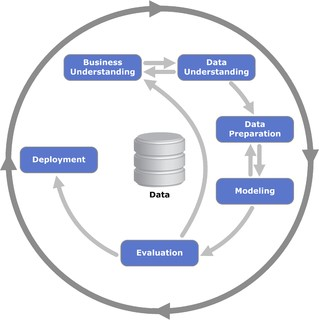
\includegraphics[width=0.46\textwidth,
                   height=0.32\textheight,
                   keepaspectratio]{images/CRISP-DM.jpg}
  \caption{Metodologi \textit{CRISP-DM}}
  \label{fig:crispdm}
\end{figure}

Metodologi pelaksanaan tugas akhir ini mengadopsi kerangka kerja CRISP-DM\label{abbr:CRISPDM} (\textit{Cross-Industry Standard Process for Data Mining}) untuk tahapan pengolahan data dan analitik. Pendekatan ini dipilih agar proses penelitian berjalan secara iteratif, fleksibel, dan tetap sistematis dalam menyelesaikan permasalahan yang telah dirumuskan.

\textbf{CRISP-DM} (\textit{Cross-Industry Standard Process for Data Mining}) adalah metodologi standar lintas industri untuk penambangan data yang menyediakan pendekatan terstruktur dalam enam fase utama, yaitu pemahaman bisnis (\textit{business understanding}), pemahaman data (\textit{data understanding}), persiapan data (\textit{data preparation}), pemodelan (\textit{modeling}), evaluasi (\textit{evaluation}), dan penyebaran (\textit{deployment}) (DataScience-PM, 2024). Metodologi ini bersifat iteratif, yang memungkinkan pengulangan fase jika diperlukan untuk meningkatkan kualitas hasil. Dalam penelitian ini, \textbf{CRISP-DM digunakan} untuk mengelola aspek penambangan data dan analitik prediktif.

\subsection{Tahapan Investigasi dan Pengumpulan Fakta}

Tahapan ini bertujuan untuk mengumpulkan data dan informasi faktual sebagai landasan perumusan masalah. Kegiatan yang dilakukan meliputi:

\begin{enumerate}[label=\alph*.]
  \item \textbf{Observasi sistem yang ada}, yaitu pengamatan terhadap sistem yang saat ini digunakan organisasi untuk mengidentifikasi keterbatasan dan kebutuhan pengguna internal.
  
  \item \textbf{Wawancara dengan pemangku kepentingan}, dilakukan secara terstruktur dengan perwakilan pemangku kepentingan internal untuk menggali kebutuhan fungsional dan ekspektasi terhadap sistem baru.
  
  \item \textbf{Analisis data historis}, dilakukan untuk menelaah volume dan tren permintaan, pola musiman, serta kelengkapan dan kualitas data yang tersedia.
  
  \item \textbf{Dokumentasi temuan}, mengompilasi seluruh hasil observasi, wawancara, dan analisis dalam bentuk laporan yang akan dilampirkan.
\end{enumerate}

\subsection{Studi Literatur}

Tahapan ini bertujuan untuk mengumpulkan, mengelompokkan, dan menyaring literatur yang relevan dengan topik penelitian. Proses yang dilakukan meliputi:

\begin{enumerate}[label=\alph*.]
  \item \textbf{Pencarian literatur sistematis} pada basis data akademik (IEEE Xplore, ScienceDirect, SpringerLink, ACM Digital Library, Google Scholar) menggunakan kata kunci terkait \textit{business intelligence}, \textit{chatbot}, \textit{natural language generation}, dan \textit{time series forecasting}. 
  
  \item \textbf{Pengelompokan literatur} berdasarkan tema utama, yaitu konsep \textit{Business Intelligence}, teknologi \textit{chatbot} dan \textit{conversational} AI, pemrosesan bahasa alami, metode peramalan deret waktu, integrasi sistem, dan studi kasus implementasi.
  
  \item \textbf{Penapisan dan analisis kualitas} literatur berdasarkan faktor dampak, jumlah sitasi, metodologi, dan relevansi terhadap penelitian.
  
  \item \textbf{Sintesis literatur} untuk membangun kerangka teoretis, mengidentifikasi praktik terbaik dan teknologi terkini, serta menyusun tinjauan pustaka pada Bab II.
  
  \item \textbf{Dokumentasi proses} dalam bentuk peninjauan penelitian terdahulu yang ditemukan dan membuat celah penelitian dan kontribusi besar yang ditawarkan penelitian ini.
\end{enumerate}

\subsection{Perancangan Sistem}

Tahapan ini meliputi perancangan arsitektur dan komponen sistem secara terperinci, mencakup:

\begin{enumerate}[label=\alph*.]
  \item \textbf{Perancangan arsitektur sistem}, yaitu penyusunan arsitektur berlapis yang mengintegrasikan \textit{chatbot}, pemrosesan bahasa alami, mesin \textit{rule-based query}, dan peramalan deret waktu, serta penentuan teknologi dan kerangka kerja yang akan digunakan.
  
  \item \textbf{Perancangan modul \textit{chatbot}}, meliputi komponen pemahaman bahasa alami (\textit{Natural Language Understanding}), manajemen dialog (\textit{Dialogue Management}), pembangkitan bahasa alami (\textit{Natural Language Generation}), serta pendefinisian \textit{intent} dan entitas yang akan dikenali.
  
  \item \textbf{Pengimplementasian \textit{rule-based query}}, yaitu pendefinisian aturan untuk kueri terstruktur dan berulang serta pemetaan antara \textit{intent} dengan templat kueri.
  
  \item \textbf{Perancangan model peramalan deret waktu}, meliputi penentuan variabel target, perancangan praolah data, pemilihan arsitektur model (ARIMA, Prophet, LSTM, dan GRU), perbandingan model statistik dengan model \textit{deep learning}, dan strategi evaluasi model.
  
  \item \textbf{Perancangan basis data dan gudang data}, yaitu perancangan skema basis data untuk menyimpan data pelanggan, hasil prediksi, dan data pelatihan NLP, serta perancangan proses ETL\label{abbr:ETL} (\textit{Extract, Transform, Load}).
  
  \item \textbf{Perancangan antarmuka pengguna}, meliputi pembuatan \textit{wireframe} dan \textit{mockup} untuk antarmuka \textit{chatbot}.
\end{enumerate}

\subsection{Implementasi Sistem}

Tahapan ini meliputi pengembangan sistem berdasarkan rancangan yang telah ditetapkan, mencakup:

\begin{enumerate}[label=\alph*.]
  \item \textbf{Pengembangan \textit{backend}}, yaitu implementasi mesin \textit{rule-based query}, model NLP untuk klasifikasi \textit{intent} dan pengenalan entitas, model peramalan deret waktu, serta penyediaan API\label{abbr:API} \textit{backend}.
  
  \item \textbf{Pengembangan \textit{frontend}}, meliputi implementasi antarmuka \textit{chatbot}.
  
  \item \textbf{Pengembangan basis data}, yaitu implementasi skema basis data, proses ETL untuk integrasi data, dan \textit{data pipeline} untuk pemrosesan data.
  
  \item \textbf{Integrasi komponen}, meliputi integrasi \textit{chatbot} dengan mesin \textit{rule-based query} dan NLP, integrasi model peramalan dengan sistem BI, serta implementasi mekanisme tembolok (\textit{caching}) untuk performa.
\end{enumerate}

\subsection{Pengujian dan Evaluasi}

Tahapan ini bertujuan menilai kinerja sistem secara menyeluruh, mencakup aspek fungsionalitas, akurasi, performa, dan kebergunaan.

\begin{enumerate}[label=\alph*.]
  \item \textbf{Pengujian unit}, yaitu setiap komponen diuji secara terpisah agar fungsinya terverifikasi dengan benar dan stabil.
  \item \textbf{Pengujian integrasi}, yaitu Interaksi antarmodul diverifikasi melalui skenario ujung-ke-ujung, dari masukan percakapan hingga keluaran berupa kueri yang dieksekusi, prediksi, narasi, dan visualisasi.
  \item \textbf{Pengujian fungsional}, yaitu Pemenuhan seluruh kebutuhan fungsional divalidasi menggunakan himpunan skenario representatif yang mencerminkan pertanyaan bisnis prioritas.
  \item \textbf{Evaluasi model NLP (klasifikasi intent multi\-kelas, satu label per ujaran)}, yaitu hasil dilaporkan sebagai \textit{top-1} dan \textit{top-k} accuracy; \textit{precision}, \textit{recall}, dan \textit{F1-score} per kelas yang kemudian dirata-ratakan dengan pendekatan \textit{macro}, \textit{micro}, dan \textit{weighted}. Disajikan pula \textit{confusion matrix} berukuran $K\times K$, evaluasi ambang kepercayaan untuk mekanisme \textit{fallback}/\texttt{UNKNOWN}, serta ringkasan kalibrasi probabilitas.
  \item \textbf{Evaluasi model peramalan deret waktu}, yaitu protokol yang digunakan ialah \textit{rolling-origin backtesting} pada beberapa horizon prediksi dengan \textit{seasonal naive} sebagai garis dasar. Laporan mencakup MAE\label{abbr:MAE}, RMSE\label{abbr:RMSE}, sMAPE\label{abbr:sMAPE}, dan MASE\label{abbr:MASE}, dilengkapi \textit{skill score} terhadap garis dasar. Hasil disajikan per horizon dan per entitas prioritas (median dan rentang antar kuartil).
  \item \textbf{Evaluasi performa sistem}, yaitu waktu respons, \textit{throughput}, dan latensi diukur pada beban realistis; \textit{load testing} dilakukan untuk menilai skalabilitas.
  \item \textbf{Evaluasi kebergunaan (\textit{usability})}, yaitu \textit{User Acceptance Testing} melibatkan sedikitnya 20–30 pengguna internal. Hasil dirangkum menggunakan skor \textit{System Usability Scale} (SUS)\label{abbr:SUS} dan umpan balik kualitatif terkait kemudahan, kejelasan, dan alur kerja.
\end{enumerate}

\subsection{Dokumentasi dan Penyusunan Laporan}

Tahapan akhir meliputi dokumentasi dan penyusunan laporan tugas akhir, mencakup:

\begin{enumerate}[label=\alph*.]
  \item \textbf{Dokumentasi teknis}, yaitu penyusunan dokumentasi API, dokumentasi kode, panduan pengguna (\textit{user manual}), dan panduan penyebaran (\textit{deployment guide}).
  
  \item \textbf{Penyusunan laporan tugas akhir}, meliputi penulisan laporan sesuai format yang ditetapkan dengan penyuntingan dan pemeriksaan kelengkapan.
  
  \item \textbf{Persiapan presentasi}, meliputi pembuatan \textit{slide} presentasi, penyusunan skenario demonstrasi sistem, dan kurasi materi pendukung.
  
  \item \textbf{Revisi dan finalisasi}, yaitu revisi berdasarkan masukan pembimbing, finalisasi laporan dan sistem, serta persiapan sidang tugas akhir.
\end{enumerate}

Seluruh proses metodologi ini akan didokumentasikan dengan baik untuk keterbukaan, kemampuan direproduksi, dan akuntabilitas penelitian.

\subsection{Sistematika Penulisan}

Laporan tugas akhir ini disusun dengan sistematika sebagai berikut.

\begin{enumerate}
  \item \textbf{Bab I Pendahuluan}: Berisi latar belakang, rumusan masalah, tujuan, batasan masalah, metodologi, dan sistematika penulisan laporan tugas akhir.
  \item \textbf{Bab II Studi Literatur}: Berisi kajian pustaka yang relevan dengan topik tugas akhir, mencakup teori dan konsep \textit{Business Intelligence}, \textit{chatbot} berbasis aturan, pemrosesan bahasa alami, pembangkitan bahasa alami, serta metode peramalan deret waktu.
  \item \textbf{Bab III Analisis}: Berisi analisis kebutuhan pengguna dan sistem, termasuk identifikasi pemangku kepentingan, kebutuhan fungsional dan non-fungsional, serta analisis data historis.
  \item \textbf{Bab IV Perancangan}: Berisi perancangan arsitektur sistem, modul \textit{chatbot} berbasis aturan, model peramalan, basis data, antarmuka pengguna, serta rencana implementasi dan evaluasi.
  \item \textbf{Bab V Implementasi}: Berisi penjelasan tentang proses implementasi seluruh komponen sistem, termasuk \textit{backend}, mesin aturan, klasifikasi maksud, pembangkitan bahasa alami, layanan \textit{machine learning}, \textit{frontend}, dan keamanan sistem.
  \item \textbf{Bab VI Evaluasi}: Berisi hasil pengujian fungsional, evaluasi akurasi model peramalan, analisis performa sistem, dan penilaian kebergunaan oleh pengguna internal.
  \item \textbf{Bab VII Kesimpulan dan Saran}: Berisi kesimpulan dari hasil pelaksanaan tugas akhir dan saran untuk pengembangan lebih lanjut.
  \item \textbf{Daftar Pustaka}: Berisi daftar referensi yang digunakan dalam penyusunan laporan tugas akhir.
  \item \textbf{Lampiran}: Berisi dokumen pendukung seperti transkrip wawancara, data pengujian, dan kode program.
\end{enumerate}



% \cleardoublepage % memastikan bab baru dimulai di halaman ganjil (kanan)
% \chapter{PENDAHULUAN}
% \label{chap:pendahuluan}
% % --- Latar Belakang ---
% \section{Latar Belakang}
% Subbab ini menjelaskan dasar pemikiran, motivasi, kebutuhan, alasan, atau urgensi pemilihan masalah tugas akhir. Subbab ini berisi penjelasan ringkas tentang kondisi atau situasi yang ada saat ini terkait dengan topik yang dibahas. Tujuan utamanya adalah untuk memberikan informasi secukupnya kepada pembaca agar memahami topik yang akan dibahas. Dalam subbab ini, jelaskan hal-hal berikut ini:
% \begin{enumerate}
% \item	Kondisi atau situasi topik yang dibahas beserta permasalahannya, misalnya tentang pengelolaan informasi di fasilitas kesehatan daerah pedesaan saat ini dan masalah yang dihadapi, berdasarkan hasil survei atau wawancara dengan pihak terkait.
% \item	Urgensi atau pentingnya penyelesaian masalah tersebut, misalnya dampak negatif yang ditimbulkan jika masalah tersebut tidak diselesaikan.
% \item	Berbagai solusi yang telah diterapkan maupun solusi yang memungkinkan untuk diterapkan untuk menyelesaikan masalah tersebut, berdasarkan hasil studi literatur, wawancara dengan pihak terkait, atau kunjungan lapangan.
% \item   Kelemahan atau kekurangan dari solusi yang telah diterapkan atau yang memungkinkan untuk diterapkan tersebut, yang menjadi dasar pemikiran dalam merumuskan masalah tugas akhir.
% \end{enumerate}
% Latar belakang dapat ditulis dalam 2-3 halaman. Penulisan latar belakang masalah yang baik akan mengantarkan pembaca kepada pemahaman yang jelas tentang topik yang akan dibahas, 
% sehingga pembaca dapat mengikuti pembahasan pada subbab-subbab berikutnya dengan baik. Oleh karena itu, 
% penulis diharapkan melakukan investigasi yang mendalam untuk mengumpulkan fakta-fakta yang relevan dengan topik yang dibahas, 
% baik melalui studi literatur, wawancara dengan pihak terkait, maupun kunjungan lapangan. Hasil studi ini dijelaskan secara \emph{ringkas} di dalam subbab ini.
% Penjelasan hasil studi literatur yang komprehensif dapat dijabarkan di Bab II Studi Literatur secara sistematis.

% Dalam menulis latar belakang, hindari penulisan yang bersifat terlalu umum atau terlalu luas cakupannya sehingga sulit untuk dihubungkan dengan topik yang dibahas dalam tugas akhir,
% seperti:
% \begin{enumerate}
%     \item "Pentingnya teknologi informasi dalam kehidupan manusia."
%     \item "Perkembangan pesat teknologi \emph{artificial intelligence} di era digital."
%     \item "Tantangan dalam pengelolaan data besar (\emph{big data}) di berbagai sektor industri."
%     \item "Peran teknologi informasi dalam meningkatkan kualitas layanan kesehatan."
% \end{enumerate}
% Penulisan yang terlalu umum atau luas cakupannya akan menyulitkan penulis dalam merumuskan masalah, tujuan, metodologi, dan evaluasi tugas akhir.

% Jika ada referensi yang digunakan dalam penulisan latar belakang, cantumkan referensi tersebut dengan benar menggunakan \texttt{biblatex} sesuai dengan contoh penulisan kutipan dan daftar pustaka yang telah disediakan dalam template ini.
% Sebagai contoh, pada paragraf berikut ini terdapat kutipan dari dua referensi yang berbeda \autocite{laudon2020, pressman2019}. 
% Ada dua format penulisan sitasi yang dapat digunakan, yaitu format naratif dan format parentetik.
% Contoh penulisan kutipan dengan format naratif adalah sebagai berikut:
% \begin{displayquote}
% Menurut \textcite{laudon2020}, sistem informasi adalah kombinasi dari teknologi informasi dan aktivitas orang yang menggunakan teknologi tersebut untuk mendukung operasi dan manajemen organisasi.
% \end{displayquote}
% Contoh penulisan kutipan dengan format parentetik adalah sebagai berikut:
% \begin{displayquote}
%     Sistem informasi merupakan kombinasi dari teknologi informasi dan aktivitas orang yang menggunakan teknologi tersebut untuk mendukung operasi dan manajemen organisasi \autocite{laudon2020}.
% \end{displayquote}
% % --- Rumusan Masalah ---
% \section{Rumusan Masalah}
% Rumusan Masalah berisi masalah utama yang dibahas dalam tugas akhir. Rumusan masalah yang baik memiliki struktur sebagai berikut:
% \begin{enumerate}
% \item	Pokok persoalan dari kondisi atau situasi yang ada saat ini. Dengan kata lain, jelaskan kelemahan atau kekurangan dari kondisi, situasi, atau solusi yang dijelaskan pada latar belakang. Ini merupakan pokok rumusan masalah.
% \item	Elaborasi lebih lanjut urgensi penyelesaian masalah tersebut (mengapa penting untuk diselesaikan dan akibat yang dapat terjadi jika tidak diselesaikan).
% \item	Usulan singkat terkait dengan solusi yang ditawarkan untuk menyelesaikan persoalan.
% Penting untuk diperhatikan bahwa persoalan yang dideskripsikan pada subbab ini akan dipertanggungjawabkan di bab Evaluasi (apakah terselesaikan atau tidak).
% \end{enumerate}
% Hindari penulisan rumusan masalah yang terlalu umum atau terlalu luas cakupannya sehingga sulit untuk diselesaikan dalam jangka waktu pelaksanaan tugas akhir, 
% seperti:
% \begin{enumerate}
%     \item "Bagaimana cara meningkatkan kualitas layanan kesehatan di Indonesia?"
%     \item "Bagaimana cara mengoptimalkan penggunaan energi di perkotaan?"
%     \item "Bagaimana cara mengurangi kemacetan lalu lintas di kota besar?"
%     \item "Bagaimana cara membangun sistem irigasi sawah menggunakan \emph{AI}?"
% \end{enumerate}
% Rumusan masalah yang baik dan spesifik akan memudahkan penulis dalam menentukan tujuan, metodologi, dan evaluasi tugas akhir.

% Selain itu, hindari menuliskan pertanyaan yang merupakan sebuah keniscayaan yang harus dijawab atau dikerjakan 
% dalam pelaksanaan tugas akhir, seperti:
% \begin{enumerate}
%     \item "Bagaimana cara melakukan analisis kebutuhan sistem informasi rumah sakit?"
%     \item "Bagaimana cara merancang basis data untuk aplikasi X?"
%     \item "Bagaimana cara mengimplementasikan \textit{large language model} untuk deteksi penyakit Y?"
%     \item "Bagaimana cara menguji sistem penyiraman tanaman berbasis IoT yang akan dibuat?"
% \end{enumerate}
% Kegiatan analisis, perancangan, implementasi, dan pengujian merupakan tahapan yang harus dilakukan dalam pelaksanaan tugas akhir,
% sehingga pertanyaan-pertanyaan tersebut tidak perlu dimasukkan ke dalam rumusan masalah.

% % --- Tujuan ---
% \section{Tujuan}
% Tuliskan \textbf{tujuan utama} dan/atau tujuan detail yang akan dicapai dalam pelaksanaan tugas akhir. 
% Fokuskan isi subbab ini pada hasil akhir yang ingin diperoleh setelah tugas akhir diselesaikan 
% terkait dengan penyelesaian persoalan pada rumusan masalah. 
% Penting untuk diperhatikan bahwa tujuan yang dideskripsikan pada subbab ini akan dipertanggungjawabkan 
% di akhir pelaksanaan tugas akhir. Oleh karena itu, tuliskan juga \emph{kriteria keberhasilan} tugas akhir ini.

% % --- Batasan Masalah ---
% \section{Batasan Masalah}
% Tuliskan batasan-batasan yang diambil dalam pelaksanaan tugas akhir. Batasan ini dapat dihindari (bersifat opsional, tidak perlu ada) jika topik atau judul tugas akhir dibuat cukup spesifik.

% % --- Metodologi Pengerjaan TA ---
% \section{Metodologi}
% Tuliskan semua tahapan yang akan dilalui selama pelaksanaan tugas akhir. 
% Tahapan ini spesifik untuk menyelesaikan persoalan tugas akhir. 
% Berikut adalah contoh metodologi pengerjaan tugas akhir yang dapat diikuti, yaitu meliputi tahapan, langkah-langkah, 
% atau tata cara melakukan:
% \begin{enumerate}
% \item	Investigasi pengumpulan fakta di latar belakang untuk merumuskan masalah.
% \item	Pencarian, pengelompokan, dan penapisan literatur atau sumber informasi untuk mengumpulkan informasi yang relevan tentang topik yang diangkat, termasuk teori (konsep atau teori apa saja yang perlu dicari), hal-hal yang telah dicapai oleh orang lain (cara mencari dan kata kuncinya), dan berbagai informasi pendukung, untuk mencari solusi terhadap masalah yang dibahas. Gunakan metodologi yang tepat dalam menggali informasi dan dokumentasikan prosesnya (termasuk rekaman wawancara atau survei) di dalam Lampiran, termasuk tautan ke video atau foto. Hasil penggalian informasi ini akan dijelaskan secara sistematis di Bab II Studi Literatur.
% \item   Analisis kebutuhan pengguna dan sistem berdasarkan hasil investigasi dan studi literatur. Jelaskan metode yang digunakan untuk melakukan analisis kebutuhan, misalnya wawancara, survei, observasi, atau studi kasus. Hasil analisis kebutuhan ini akan dijelaskan secara rinci di Bab III Analisis.
% \item   Perancangan solusi berdasarkan hasil analisis kebutuhan. Jelaskan metode yang digunakan untuk melakukan perancangan, misalnya menggunakan diagram UML, ERD, atau prototyping. Hasil perancangan ini akan dijelaskan secara rinci di Bab IV Perancangan.
% \item   Implementasi solusi berdasarkan hasil perancangan. Jelaskan teknologi, bahasa pemrograman, atau alat yang digunakan untuk mengimplementasikan solusi. Hasil implementasi ini akan dijelaskan secara rinci di Bab V Implementasi.
% \item   Evaluasi terhadap solusi yang telah diimplementasikan. Jelaskan metode pengujian, metrik evaluasi, atau studi kasus yang digunakan untuk menilai keberhasilan solusi. Hasil evaluasi ini akan dijelaskan secara rinci di Bab VI Evaluasi.
% \item   Penarikan kesimpulan dan saran berdasarkan hasil pelaksanaan tugas akhir. Hasil kesimpulan dan saran ini akan dijelaskan secara rinci di Bab VII Kesimpulan dan Saran. 
% \vfill % memaksa konten di atas untuk berada di bagian atas halaman dan menyisakan ruang kosong di bawah konten ini akibat berakhirnya section ini
% \end{enumerate}

% % --- Sistematika Penulisan ---
% \section{Sistematika Penulisan}
% Tuliskan gambaran umum isi dari setiap bab yang ada dalam laporan tugas akhir. Sistematika penulisan ini memberikan panduan bagi pembaca tentang struktur dan alur pembahasan dalam laporan tugas akhir. Berikut adalah contoh sistematika penulisan yang dapat diikuti:
% \begin{enumerate}
% \item	Bab I Pendahuluan: Berisi latar belakang, rumusan masalah, tujuan, batasan masalah, metodologi, dan sistematika penulisan laporan tugas akhir       .
% \item	Bab II Studi Literatur: Berisi kajian pustaka yang relevan dengan topik tugas akhir, termasuk teori-teori, konsep-konsep, dan hasil-hasil penelitian sebelumnya yang                mendukung pelaksanaan tugas akhir.
% \item	Bab III Analisis: Berisi penjelasan tentang analisis masalah dan kebutuhan pengguna serta berbagai alternatif solusinya.
% \item   Bab IV Perancangan: Berisi penjelasan tentang perancangan solusi yang diusulkan, misalnya arsitektur sistem, desain basis data, antarmuka pengguna, dan sebagainya.
% \item	Bab V Implementasi: Berisi penjelasan tentang proses implementasi solusi yang diusulkan, termasuk langkah-langkah yang diambil, teknologi yang digunakan, dan hasil yang diperoleh.
% \item	Bab VI Evaluasi: Berisi analisis dan evaluasi terhadap solusi yang diimplementasikan, termasuk metode pengujian, hal-hal yang disiapkan sebelum pengujian, hasil pengujian, dan penilaian kinerja.                  
% \item   Bab VII Kesimpulan dan Saran: Berisi kesimpulan dari hasil pelaksanaan tugas akhir dan saran untuk pengembangan lebih lanjut.
% \item   Daftar Pustaka: Berisi daftar referensi yang digunakan dalam penyusunan laporan tugas akhir.
% \item   Lampiran: Berisi dokumen-dokumen pendukung seperti kode program, data lengkap hasil pengujian, rekaman wawancara, dan lain-lain. 
% \end{enumerate}